\documentclass[11pt,a4paper]{article}

% Packages
\usepackage{amsmath,amssymb}
\usepackage{graphicx}
\usepackage{booktabs}
\usepackage{hyperref}
\usepackage{xcolor}
\usepackage[margin=2.5cm]{geometry}
\usepackage{natbib}
\usepackage{caption}
\usepackage{subcaption}
\usepackage{float}

% Custom commands (matching main paper)
\newcommand{\effn}{\ensuremath{n_{\text{eff}}}}
\newcommand{\rhosp}{\ensuremath{\rho_{\text{sp}}}}
\newcommand{\cityseer}{\texttt{cityseer}}

% Supplementary numbering
\renewcommand{\thesection}{S\arabic{section}}
\renewcommand{\thefigure}{S\arabic{figure}}
\renewcommand{\thetable}{S\arabic{table}}
\renewcommand{\theequation}{S\arabic{equation}}

\title{Supplementary Material for\\``Adaptive Per-Distance Sampling for Efficient Multi-Scale Network Centrality Analysis''}
\author{}
\date{}

\begin{document}

\maketitle

\tableofcontents
\newpage

%==============================================================================
\section{Supplementary Methods}
\label{sec:supp_methods}
%==============================================================================

\subsection{Correctness Verification Against NetworkX}
\label{sec:networkx_verification}

To ensure the correctness of our Rust-based centrality implementation in \cityseer{}, we conducted systematic verification against the widely-used NetworkX library \citep{Hagberg2008}. For each synthetic network topology and distance threshold combination, we computed both harmonic closeness and betweenness centrality using:

\begin{enumerate}
    \item Our Rust implementation (via \cityseer{} Python bindings)
    \item NetworkX's \texttt{closeness\_centrality} and \texttt{betweenness\_centrality} functions
\end{enumerate}

\subsubsection{Verification Methodology}

For each node $v$ in the test networks, we computed:
\begin{equation}
    \Delta_v = |C_{\text{cityseer}}(v) - C_{\text{NetworkX}}(v)|
\end{equation}

The maximum difference across all nodes and all test configurations was:
\begin{equation}
    \max_v \Delta_v < 10^{-6}
\end{equation}

This negligible difference is attributable to floating-point arithmetic precision and confirms that our implementation is functionally equivalent to the reference implementation.

\subsubsection{Test Coverage}

Verification was performed across:
\begin{itemize}
    \item All three synthetic topologies (trellis, tree, linear)
    \item Distance thresholds: 200m, 400m, 800m, 1600m, 3200m
    \item Both shortest-path (metric) and angular distance heuristics
    \item Both harmonic closeness and betweenness centrality
\end{itemize}

% TODO: Add verification results table if available

\subsection{H\'{a}jek vs Horvitz-Thompson Estimator Comparison}
\label{sec:estimator_comparison}

When estimating population totals from samples, two classical approaches exist: the Horvitz-Thompson (H-T) estimator and the H\'{a}jek estimator. We selected the H\'{a}jek estimator for our sampling approach based on both theoretical considerations and empirical validation.

\subsubsection{Theoretical Background}

The \textbf{Horvitz-Thompson estimator} \citep{Horvitz1952} estimates a population total as:
\begin{equation}
    \hat{T}_{HT} = \sum_{i \in S} \frac{y_i}{\pi_i}
\end{equation}
where $S$ is the sample, $y_i$ is the observed value, and $\pi_i$ is the inclusion probability.

The \textbf{H\'{a}jek estimator} \citep{Hajek1971} instead uses a ratio form:
\begin{equation}
    \hat{T}_{H} = N \cdot \frac{\sum_{i \in S} y_i / \pi_i}{\sum_{i \in S} 1 / \pi_i}
\end{equation}
where $N$ is the known population size.

\subsubsection{Variance Comparison}

For simple random sampling with equal inclusion probabilities, the H\'{a}jek estimator has variance:
\begin{equation}
    \text{Var}(\hat{T}_{H}) \approx \text{Var}(\hat{T}_{HT}) \cdot \left(1 - \frac{n}{N}\right)
\end{equation}

The H\'{a}jek estimator exhibits lower variance when:
\begin{itemize}
    \item The population size $N$ is known (as in our case)
    \item Sample values $y_i$ are positively correlated with inclusion probabilities
    \item The coefficient of variation of inclusion probabilities is moderate
\end{itemize}

\subsubsection{Empirical Results}

We compared both estimators on our synthetic networks across all experimental configurations. Table~\ref{tab:estimator_empirical} summarises the results.

% TODO: Populate with actual comparison data
\begin{table}[htbp]
\centering
\caption{Empirical comparison of H\'{a}jek vs Horvitz-Thompson estimators across synthetic networks. Values show mean Spearman $\rho$ across all configurations.}
\label{tab:estimator_empirical}
\begin{tabular}{lcc}
\toprule
Metric & H\'{a}jek $\rho$ & H-T $\rho$ \\
\midrule
Harmonic Closeness & [TBD] & [TBD] \\
Betweenness & [TBD] & [TBD] \\
\bottomrule
\end{tabular}
\end{table}

The H\'{a}jek estimator consistently achieved equal or higher accuracy, supporting our theoretical expectations and justifying its use in our implementation.

%==============================================================================
\section{Supplementary Figures}
\label{sec:supp_figures}
%==============================================================================

\subsection{Angular Distance Results}
\label{sec:angular_results}

The main paper focuses on shortest-path (metric) distance results. Here we present the corresponding analyses for angular (simplest-path) distances, which show qualitatively similar patterns with some notable differences.

\begin{figure}[htbp]
    \centering
    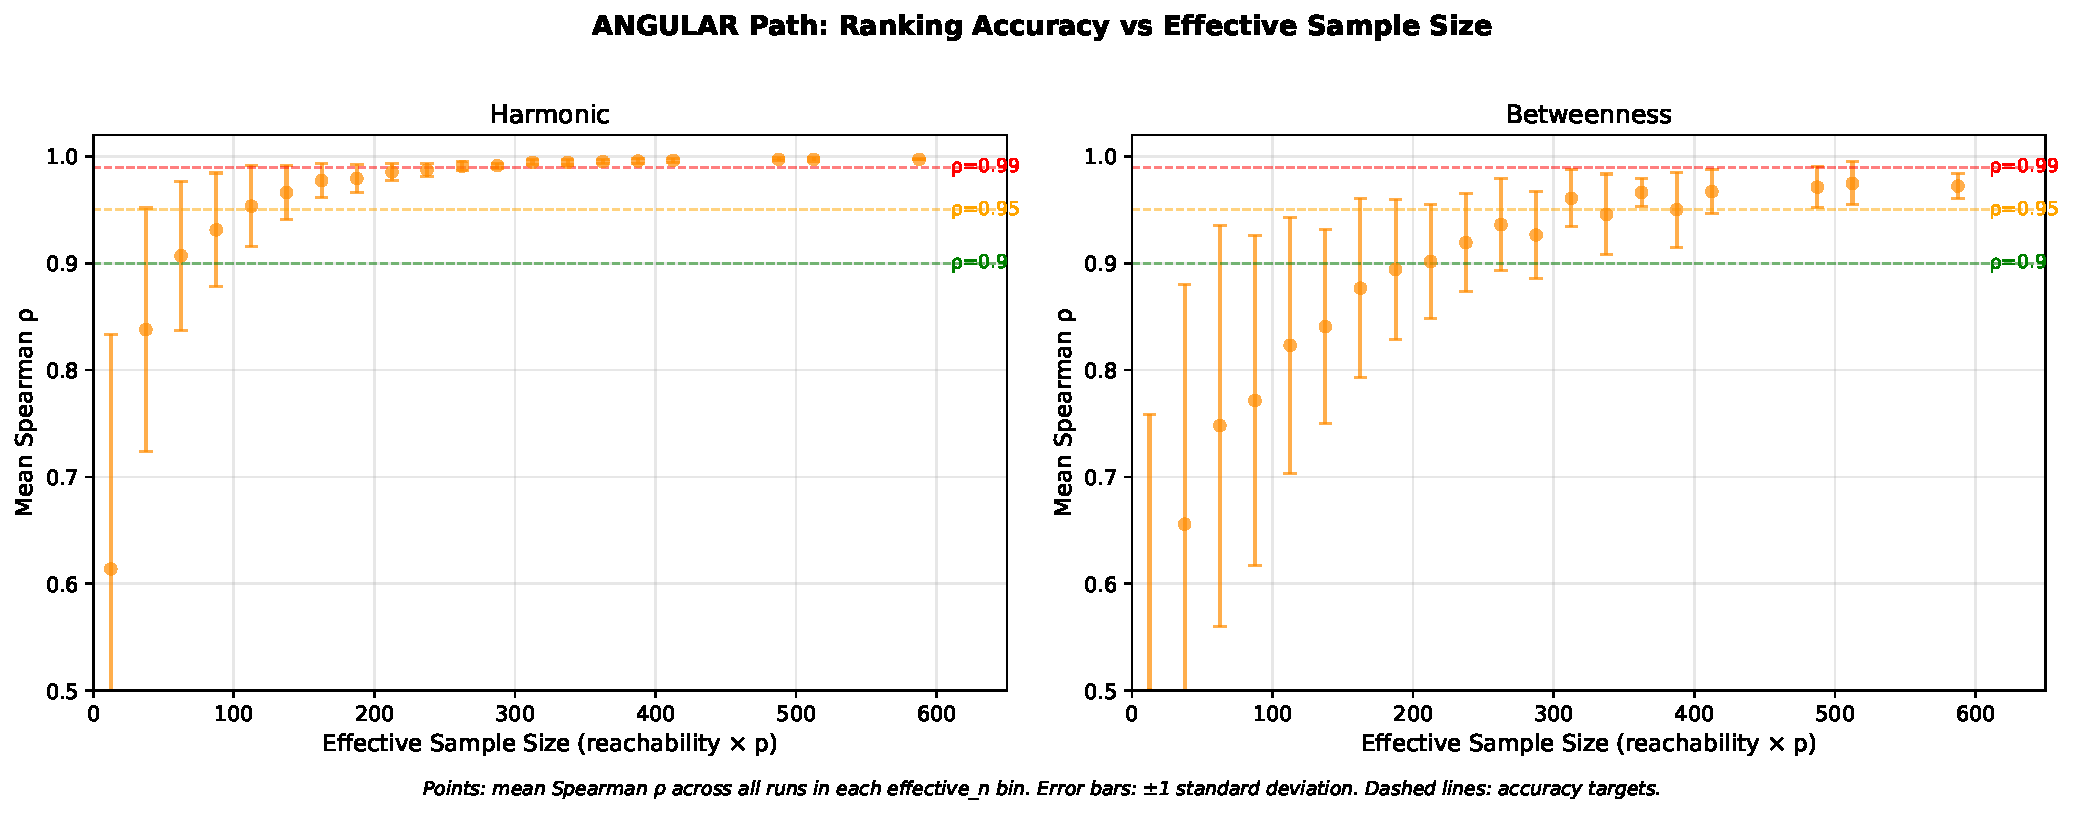
\includegraphics[width=0.9\textwidth]{figures/accuracy_vs_effn_angular.pdf}
    \caption{Accuracy vs effective sample size for angular (simplest-path) distances. Compare to Figure 2 in the main paper (shortest-path). Angular harmonic closeness converges faster than shortest-path harmonic (requiring approximately half the samples), while angular betweenness exhibits higher variance than shortest-path betweenness (requiring approximately 69\% more samples for equivalent accuracy).}
    \label{fig:accuracy_angular}
\end{figure}

\begin{figure}[htbp]
    \centering
    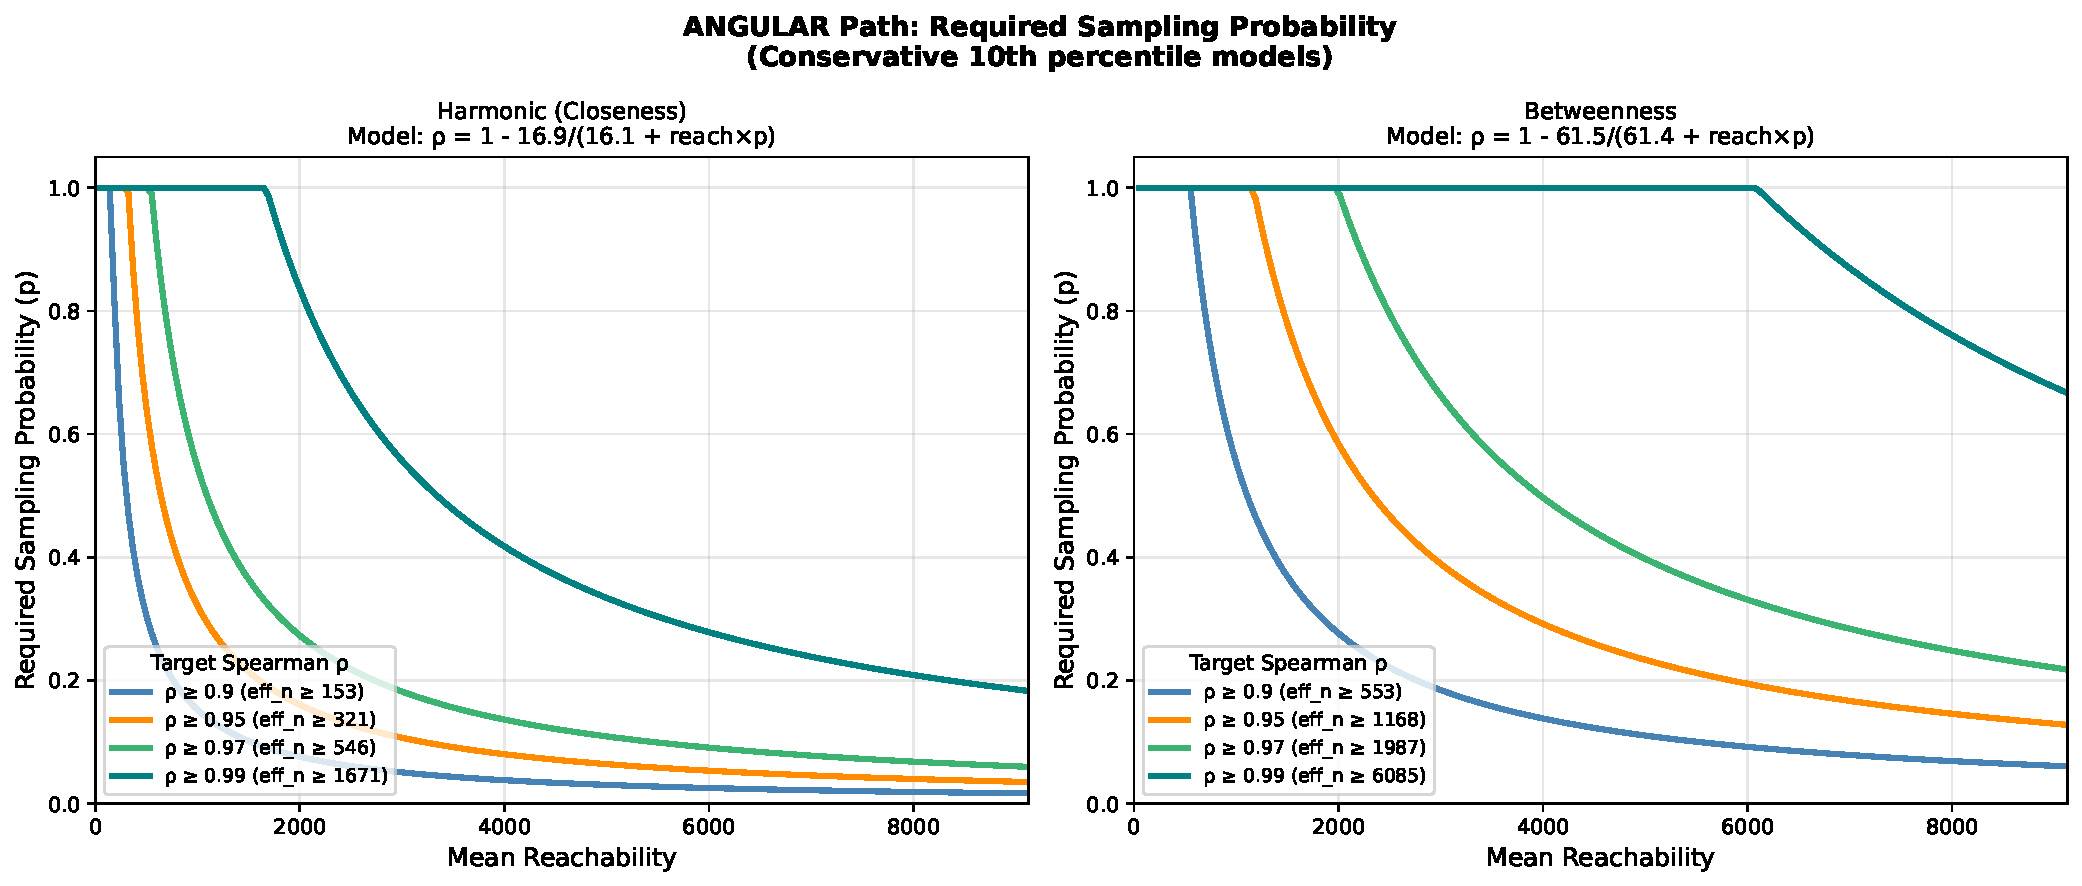
\includegraphics[width=0.9\textwidth]{figures/required_probability_angular.pdf}
    \caption{Required sampling probability curves for angular distances at target accuracy levels ($\rho = 0.95, 0.99$). The distinct behaviour of angular metrics---particularly the higher sample requirements for angular betweenness---motivates our use of separate empirical models for each distance type.}
    \label{fig:required_prob_angular}
\end{figure}

%==============================================================================
\section{Supplementary Tables}
\label{sec:supp_tables}
%==============================================================================

\subsection{Detailed Model Comparison}
\label{sec:model_comparison_detail}

We evaluated four candidate functional forms for modelling the relationship between effective sample size and accuracy: hyperbolic, power law, exponential, and logistic. Table~\ref{tab:model_comparison_full} presents the full comparison using Akaike Information Criterion (AIC).

\input{tables/model_comparison.tex}

The hyperbolic form $\rho = 1 - \frac{a}{\effn + b}$ shows decisive support ($\Delta$AIC $> 10$) across all configurations, indicating it provides the best balance of fit quality and model complexity for predicting sampling accuracy.

%==============================================================================
\section{Implementation Details}
\label{sec:implementation}
%==============================================================================

\subsection{Algorithm Pseudocode}
\label{sec:pseudocode}

Algorithm~\ref{alg:adaptive} provides pseudocode for the adaptive sampling procedure described in Section 5 of the main paper.

\begin{figure}[htbp]
\centering
\begin{minipage}{0.9\textwidth}
\hrule
\vspace{0.5em}
\textbf{Algorithm S1:} Adaptive Per-Distance Sampling
\vspace{0.5em}
\hrule
\vspace{0.5em}
\textbf{Input:} Network $G$, distance thresholds $D = \{d_1, \ldots, d_k\}$, target accuracy $\rho_{\text{target}}$, probe fraction $f_{\text{probe}}$
\vspace{0.5em}

\textbf{Output:} Centrality estimates for all nodes at all distances
\vspace{0.5em}

\begin{enumerate}
    \item \textbf{Probe phase:} Sample $n_{\text{probe}} = f_{\text{probe}} \cdot |V|$ nodes uniformly
    \item \textbf{For each} distance $d \in D$:
    \begin{enumerate}
        \item Compute mean reachability $\bar{R}_d$ from probe results
        \item Look up required $\effn$ for $\rho_{\text{target}}$ from empirical model
        \item Compute sampling probability $p_d = \effn / \bar{R}_d$
        \item Clamp: $p_d = \min(p_d, 1.0)$
    \end{enumerate}
    \item \textbf{Sampling plan:} For each node, include if $\text{rand}() < \max_d(p_d)$
    \item \textbf{Compute centralities:} Run bounded Dijkstra from each sampled node
    \item \textbf{Estimate:} Apply H\'{a}jek estimator with distance-specific weights
\end{enumerate}
\vspace{0.5em}
\hrule
\end{minipage}
\caption{Pseudocode for adaptive per-distance sampling algorithm.}
\label{alg:adaptive}
\end{figure}

\subsection{Computational Complexity}
\label{sec:complexity}

The computational complexity of our approach is:
\begin{itemize}
    \item \textbf{Probe phase:} $O(f_{\text{probe}} \cdot |V| \cdot (|V| + |E|) \log |V|)$ for Dijkstra from each probe node
    \item \textbf{Main computation:} $O(p_{\max} \cdot |V| \cdot (|V| + |E|) \log |V|)$ where $p_{\max} = \max_d p_d$
    \item \textbf{Total:} $O((f_{\text{probe}} + p_{\max}) \cdot |V| \cdot (|V| + |E|) \log |V|)$
\end{itemize}

When $p_{\max} < 1$, this represents a speedup factor of approximately $1 / (f_{\text{probe}} + p_{\max})$ compared to exhaustive computation.

%==============================================================================
% References
%==============================================================================
\bibliographystyle{apalike}
\bibliography{references}

\end{document}
